\documentclass[conference]{IEEEtran}
\usepackage{cite}
\usepackage{graphicx}
\usepackage{amsmath,amssymb}
\usepackage{algorithm}
\usepackage{algorithmic}
\usepackage{url}
\usepackage{booktabs}
\usepackage[font=footnotesize]{subcaption}

% *** START DOCUMENT ***
\begin{document}

% Title Section
\title{Assignment 4: Random Forest Analysis of Tree Size}

\author{
\IEEEauthorblockN{Grant Booysen 25849646}
\IEEEauthorblockA{Email: 25849646@sun.ac.za}
}

\maketitle

% Abstract

\begin{abstract}
The report investigates how Random Forest performance varies with decision-tree depth, the number of randomly selected features per split, and ensemble size across three classification datasets of increasing complexity. The goal is to track the performance from underfitting with very shallow trees and few features to overfitting with deep trees and many features, identify points that maximize generalization, and characterize interactions among these hyperparameters. Experiments with (i) maximum depth from minimal to deep trees, (ii) number of features to split on with depth fixed at the best value from (i), and (iii) the balance number of trees with depth were conducted. A final experiment creates ensembles that mix under- and overfitting trees. Models are evaluated with train/test accuracy and 5-fold cross-validation. Findings are consistent: increased depth improves test accuracy up to a point, after which performance degrades or stagnates and the optimal depth increases with problem complexity. With depth fixed, increased number of features per split improves performance up to a plateau where medium complexity favors moderate feature subsets, while complex data benefits from larger subsets. The inclusion of more trees in the ensemble improves stability and accuracy up to a plateau, with gains moderated by tree depth. Bagging with only overfitted trees proved to have either the best stability, cross validation accuracy or test accuracy across all three datasets. 

  Overall, the best configurations balance depth, feature subsampling, and ensemble size where larger values are generally preferred as 
  task complexity rises. 
\end{abstract}


% Keywords (optional)
\begin{IEEEkeywords}
Random Forest, Ensemble learning, Bagging, Decision Trees
\end{IEEEkeywords}


\section{Introduction}

Random forests are widely used for classification due to strong generalization, robustness, and modest tuning requirements. The random forest model's performance is controlled by key hyperparameters that trade off bias and variance such as: maximum decision-tree depth, the number of randomly selected features per split, and ensemble size. The report aims to provide understanding for how these controls move the model to better performance. The idea is to identify configurations that generalize across problem complexities.\\

The goal of this study is to characterize how tree depth and feature subsampling influence random forest performance, and to identify configurations that maximize test accuracy and cross-validated performance across datasets of increasing difficulty. The analysis is achieved by: (i) exploring maximum depth from minimal to deep trees at fixed ensemble size, number of random features per split, and bagging; (ii) fixing depth at the best value from (i) and exploring the optimal number of features to split on per node; (iii) exploring depth and ensemble-size interactions; and (iv) composing ensembles that intentionally mix underfitted and overfitted trees. Evaluation uses train/test accuracy and 5-fold cross-validation to better assess generalization and stability.\\

The report aims to provide a reproducible behaviour for the bias-variance trade-off for random forests, and to extract 
generalizations for hyperparameter selection that adapts to dataset complexity. The design follows controlled experiments to reveal how each hyperparameter influences performance, and how they interact. The analysis spans three synthetic datasets of increasing complexity to assess how optimal configurations shift with task difficulty.\\

The main observations are consistent with the bias-variance expectations. Increasing the depth of the trees in the ensemble improves test accuracy up to a point, after which gains stagnate or degrade; the optimal depth increases with complexity, for example, approximately 8, 15, and 20 on the simple, medium, and complex datasets respectively. With depth fixed, increasing the number of features to split on improves performance then plateaus; moderate subsets suit medium complexity, while larger subsets benefit complex data. Adding trees improves stability and accuracy up to a plateau, where the number of trees needed to reach the plateau is dependent on the depth of the trees. Mixed-depth and only overfit ensembles: on the simple dataset, the highest test accuracy was 0.960 with a tie between the balanced and only overfit compositions, while only overfit attained the best cross-validated score of 0.966; on the medium dataset, the only-overfit composition achieved both the highest test accuracy of 0.685 and the best cross-validated score of 0.691; on the complex dataset, only overfitted trees achieved the highest test accuracy of 0.610 and the most stable cross-validation, with majority overfitted exhibiting a marginally higher CV mean of 0.564 versus 0.563 for only overfit.\\

The remainder of the report is organized as follows: Section~2 provides background; Section~3 details the methodology and implementation; Section~4 describes the empirical procedure; Section~5 presents results and discussion; Section~6 concludes with implications and future directions.

\section{Background}
The background section discusses the fundamental concepts and algorithms used in the report, including decision trees, ensemble learning, and 
random forests.

\subsection{Decision Trees}
The decision tree is a supervised learning algorithm used for classification and regression tasks. The decision tree works by recursively 
splitting the data into subsets based on feature values, creating a tree-like model of decisions. Each internal node represents a condition on a 
feature, each branch represents the outcome of the test, and each leaf node represents a class label in classification or a continuous value 
in regression. Decision trees are easy to interpret and visualize, but they can be prone to overfitting, especially with deep trees.

\subsection{Ensemble Learning: Bagging}
Bagging, or Bootstrap Aggregating, is an ensemble learning technique that aims to improve the stability and accuracy of machine learning algorithms.
 The algorithm works by training multiple models on different subsets of the training data, which are created by randomly sampling with 
 replacement known as bootstrapping. The final prediction is made by aggregating the predictions of all individual models, typically by 
 averaging for regression or majority voting for classification. Bagging helps reduce variance and combat overfitting, making the approach 
 particularly effective for high-variance models like decision trees.

\subsection{Random Forests}

Random forests are an ensemble learning method that combines multiple decision trees to improve predictive performance and control 
overfitting. The key idea is to leverage the diversity of individual trees by training them on different subsets of the data and features. Traditionally,
random forests use bagging to create diverse training sets for each tree. In random forests, it is expected that each tree should be grown
to the maximum depth and overfit. The high variance of each tree is then averaged out by the ensemble, leading to a final model that generalizes well.

\begin{algorithm}[H]
\caption{Random Forest (high-level pseudocode)}
\begin{algorithmic}[1]
\REQUIRE Training data $(X, y)$, n\_estimators, max\_depth, max\_features, bootstrap size
\FOR{each tree $t = 1 \dots$ n\_estimators}
  \STATE Draw a bootstrap sample from $(X, y)$  % bagging
  \STATE Grow a decision tree with depth limit max\_depth
  \STATE At each node, consider max\_features randomly selected features
\ENDFOR
\STATE For prediction, average class probabilities (or majority vote) across trees
\end{algorithmic}
\end{algorithm}

\subsection{Statistical comparison of models}
To compare multiple model configurations evaluated on the same data partitions, non-parametric, paired statistical tests are used:
\begin{itemize}
  \item \textbf{Friedman test}: compares $k$ related treatments across $N$ blocks by ranking methods within each block and testing the null hypothesis that their median ranks are equal. It avoids normality assumptions and is appropriate for repeated-measures cross-validation.
  \item \textbf{Wilcoxon signed-rank test}: conducts a paired comparison between two configurations across the same blocks. A one-sided alternative tests whether a reference method such as ``Only Overfit'' tends to outperform a comparator. Holm correction controls the family-wise error rate over multiple pairwise tests.
\end{itemize}
These tests operate on cross-validated fold scores, respect pairing, and avoid using the held-out test split for model selection.


\section{Implementation}
The implementation section describes the datasets, data preparation, and the random forest model used in the experiments.

\subsection{Data preparation}
Three synthetic, tabular classification datasets of increasing complexity were programmatically generated using 
\texttt{make\_classification} from \texttt{sklearn.datasets} \cite{scikit-learn} to enable controlled bias-variance studies and avoid confounds from missing values or categorical encoding. A single \texttt{random\_state} ensured reproducibility for generation and splitting.

\textbf{Datasets:}
\begin{itemize}
  \item Simple: binary classification, low noise, no overlap between classes, \texttt{n\_samples=500}, \texttt{n\_features=10} where eight are informative and two are redundant, \texttt{class\_sep=2.0}, \texttt{flip\_y=0.0}. Designed to saturate quickly with shallow trees and show limited overfitting.
  \item Medium: three classes, moderate overlap, mild noise, \texttt{n\_samples=2000}, \texttt{n\_features=25} where 18 are informative and five are redundant, \texttt{class\_sep=1.0}, \texttt{flip\_y=0.2}. Targets visible bias-variance trade-offs at medium depths.
  \item Complex: four classes, many features, higher noise, \texttt{n\_samples=6000}, \texttt{n\_features=50} where 35 are informative and ten are redundant, \texttt{class\_sep=0.7}, \texttt{flip\_y=0.3}. Encourages deeper trees and progressive overfitting.
\end{itemize}

\textbf{Train/test split:} A stratified split with \texttt{test\_size=0.30} and fixed \texttt{random\_state} preserves 
class proportions across splits and guarantees identical partitions across runs.


\textbf{Preprocessing:} No scaling or normalization is applied as decision trees are insensitive to monotonic feature transforms. No imputation is
 required as the synthetic data contain no missing values. No label encoding is needed as the labels are already integers.

\textbf{Depth ranges for experimental control:} Per-dataset depth grids are predefined to bound sweeps and reflect expected capacity needs:


\subsection{Random forest Model}

A custom scikit-learn compatible estimator was implemented by extending \texttt{BaseEstimator} and \texttt{ClassifierMixin}. Each base learner is a \texttt{DecisionTreeClassifier}. The 
ensemble exposes the hyperparameters: \texttt{n\_estimators}, \texttt{max\_depth}, \texttt{max\_features} (per-split random subspace), \texttt{bootstrap}, \texttt{criterion}, 
\texttt{min\_samples\_*}, \texttt{max\_leaf\_nodes}, and \texttt{ccp\_alpha}. These parameters allow control over tree complexity and randomness. Each individual tree needed 
to be able to be individually controlled to allow for the mixed underfit/overfit experiments.

Training uses standard bagging: for each tree, a bootstrap sample is drawn. A distinct, reproducible random seed is generated per tree from a generator seeded by the estimator's random seed. Each tree \texttt{max\_features} parameter enforces feature sub-sampling at each split, mirroring the random subspace mechanism. Prediction averages class probabilities across trees uses majority vote.

The model has the following characteristics:
\begin{itemize}
  \item Equal-weight averaging across trees with no out-of-bag estimates or class weighting by default.
  \item No post-hoc pruning as overfitting is intentionally permitted to study depth effects.
  \item Deterministic behavior controlled by a random seed.
\end{itemize}


\subsection{Cross-validation procedure}
Across all experiments, performance for each hyperparameter setting was estimated with K-fold stratified cross-validation on the training split only using \texttt{StratifiedKFold} from \texttt{sklearn.model\_selection} \cite{scikit-learn}, 
reporting the mean and standard deviation of accuracy. Concretely, for the tree-depth, feature-selection, and depth by trees grids, stratified folds for classification were used to compute cross-validated accuracy scores, and record CV mean and CV std. The held-out test split is evaluated separately to provide a single final generalization number, but not to select hyperparameters. Where an optimal depth is required to center configurations, the depth is chosen by maximizing the CV mean from the prior depth experiment.

\subsection{Statistical testing protocol}
For each dataset, repeated stratified K-fold cross-validation with 5 folds and 7 repeats provides fold-wise accuracies for each of the five ensemble compositions. The Friedman test serves as an omnibus check for any differences among configurations. When significant, one-sided Wilcoxon signed-rank tests compare the ``Only Overfit'' configuration against each alternative, with Holm-adjusted $p$-values to control family-wise error. Unless stated otherwise, the significance level is set to $\alpha=0.05$, and post-hoc rejections are determined by comparing Holm-adjusted $p$-values against $\alpha$.


\section{Empirical Procedure}

The emperical procedure section details the datasets, performance measures, control parameters, and the four experiments executed to answer the study goals. All experiments are fully 
reproducible given the seeds and grids below.

\subsection{Benchmarks and Splitting}
The three datasets Simple, Medium, and Complex were generated as described in the Data Preparation section. Each dataset was split into a training set at a 70\% split and a held-out test set at a 30\% split using a stratified split to maintain class proportions.

\subsection{Performance Measures and Validation}
The primary metric used was accuracy and was reported for train, test, and 5-fold stratified cross-validation on the training split. For each configuration, the following are 
recorded: train accuracy, test accuracy and CV mean and standard deviation. 

\subsection{Implementation and Controls}
A global seed of 42 was used. Per-tree seeds are drawn from a generator seeded by this value to ensure determinism. Unless varied explicitly, defaults for the 
decision trees are:
\begin{itemize}
  \item Criterion for split quality is the \texttt{gini} impurity.
  \item Minimum samples to split a node is two.
  \item Minimum samples per leaf is one.
  \item No pruning.
  \item Bootstrap sampling.
  \item Equal weighting across trees.
\end{itemize}

\textbf{Dataset-specific depth grids:} Each dataset has a predefined grid of maximum depths to explore, reflecting expected capacity needs:
\begin{itemize}
  \item Simple: \{1, 2, 3, 4, 5, 6, 8, 10, 12\}
  \item Medium: \{1, 3, 5, 7, 10, 12, 15, 18, 20, 25, 30\}
  \item Complex: \{1, 3, 5, 7, 10, 12, 15, 20, 25, 30, 35, 40\}
\end{itemize}

\subsection{Cross-validation for Experiments}
All experiments use 5-fold stratified cross-validation on the training split (StratifiedKFold). For each hyperparameter configuration we report the cross-validation mean and standard deviation, and rebuild models or ensembles within each fold when applicable. The held-out test split is evaluated separately to report train and test accuracy. The same reproducible controls (global random seed, per-tree seeds, stratified splits) apply across all experiments.

\subsection{Experiment 1: Maximum Tree Depth}
The objective of Experiment 1 is to isolate the effect of maximum tree depth on generalization and overfitting. To this end, we sweep the maximum depth from 
very shallow to very deep trees while holding other factors constant: a forest of decision trees is trained and all features are used at 
each split so that each tree is as strong as possible. The variable is the maximum depth, swept over the dataset-specific grids defined above.

\subsection{Experiment 2: Number of Features per Split}
The objective is to quantify the effect of per-split feature subsampling while holding depth near the optimal values found in Experiment~1. The experiment fixes the maximum depth to 
the CV optimal values (Simple: \texttt{max\_depth=8}, Medium: \texttt{max\_depth=15}, Complex: \texttt{max\_depth=20}), enables bagging with 30, 60, and 90 trees for the Simple, Medium, 
and Complex datasets respectively to stabilise results, and sweeps the maximum number of features per split over \{1,2,3,5,7,10,15,20,25,30,35,40,45,50\}, skipping values that 
exceed each dataset's dimensionality.
\subsection{Experiment 3: Depth vs Number of Trees}
The objective is to study the interaction between ensemble size and tree depth. In this experiment the number of features considered per split is fixed
 to \texttt{max\_features='sqrt'} to provide a moderate level of randomness and bagging is enabled. Tree depth is swept over the dataset-specific depth grids while the number of
  trees is varied per dataset. Results are visualized as heatmaps of test accuracy on the depth by number of trees grid to quantify how increasing the number of trees reduces variance up to a plateau and how the benefit of additional trees depends on tree depth. Cross-validation mean and standard deviation are reported as described above.

\subsection{Experiment 4: Mixed-Depth Ensembles}
This experiment evaluates ensembles that mix underfitting and overfitting trees to probe bias-variance blending. Controls are fixed where the number of features per split is set to the optimal values from Experiment 2, ensemble sizes and per-dataset maximum tree depths use the optima from Experiment 3, and bagging is enabled. 
Five ensemble compositions are compared:
\begin{itemize}
  \item all underfitted;
  \item majority underfitted (75\% underfitted, 25\% overfitted);
  \item balanced (50/50);
  \item majority overfitted (25\% underfitted, 75\% overfitted);
  \item all overfitted. 
\end{itemize}
Underfitted depths are sampled from depths below the optimal and overfitted depths from just above the optimal up to the maximum. The goal is to determine whether mixing tree capacities yields improved generalization or stability compared to homogeneous ensembles of the same size.



\section{Research Results}

\label{sec:results}

This section reports results for all four experiments. For each configuration the cross-validated accuracy mean and standard deviation over 5 folds on the training split and the held-out test accuracy are reported. 



\subsection{Experiment 1: Maximum Tree Depth}
\label{sec:results-exp1}

Across datasets, increasing maximum depth initially raises both CV and test accuracy as shallow ensembles underfit. Beyond dataset-specific optima, test/CV curves plateau. The figures highlight this bias-variance trade-off and localize the depth that maximizes generalization for each dataset.

\begin{figure}[H]
  \centering
  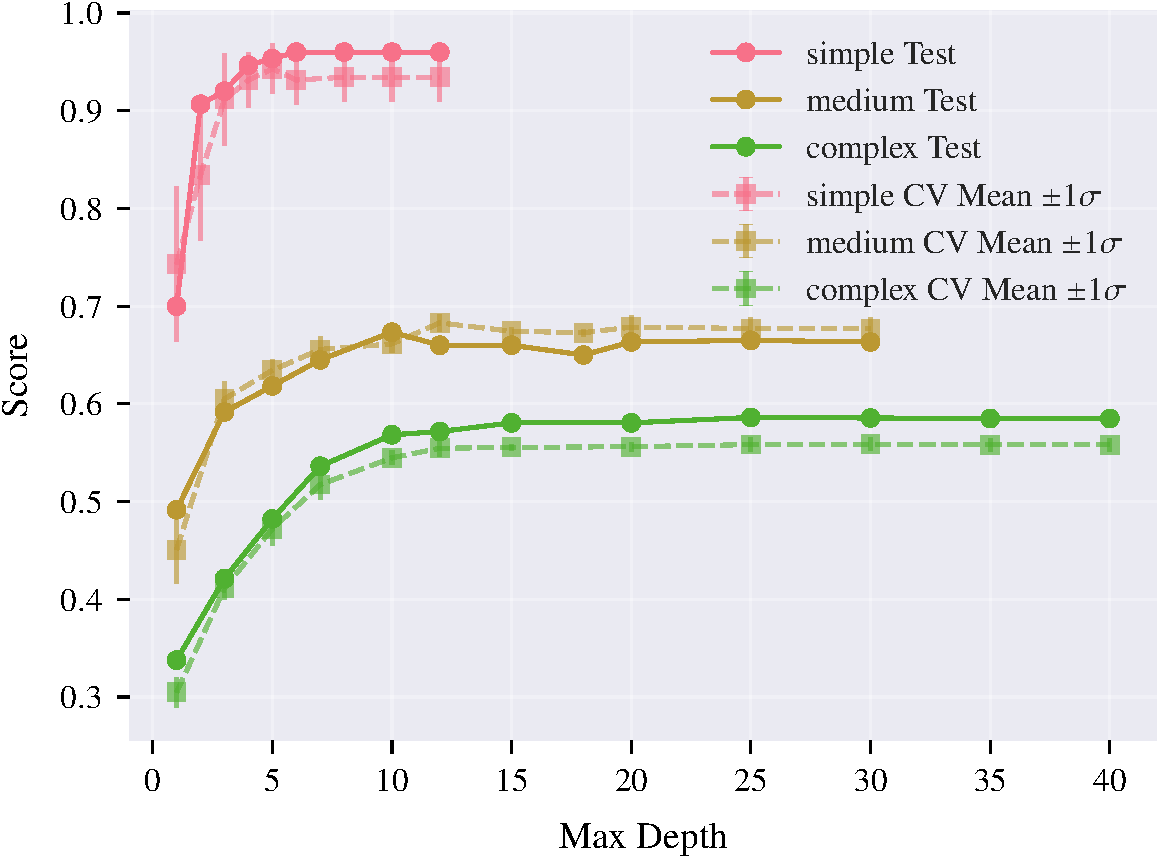
\includegraphics[width=\linewidth]{images/all_datasets_depth_accuracy.pdf}
  \caption{Maximum tree depth vs. test and cross-validated accuracy for the three datasets.}
  \label{fig:exp1-depth-acc}
\end{figure}

\textbf{Discussion:}
 The results in Figures~\ref{fig:exp1-depth-acc} show the relationship between maximum tree depth and both test and cross-validated accuracy. As expected, very shallow trees in the ensemble underfit the data, which results in low accuracy on both training and test sets. As depth increases, accuracy improves significantly, indicating that the model is capturing more complex patterns in the data. However, beyond a certain depth for example,  depth 8 for Simple, 15 for Medium, and 20 for Complex, the test accuracy plateaus or slightly decreases while training accuracy continues to rise. This indicates overfitting, where the model learns noise in the training data rather than generalizable patterns. The optimal depths identified align with the complexity of each dataset, with more complex datasets requiring deeper trees to capture their structure. These results occur due to the bias-variance trade-off inherent in decision trees. Shallow trees have high bias and low variance, leading to underfitting, while deep trees have low bias and high variance, leading to overfitting. The ensemble averages out some the variance of the overfitted individual trees. However, if there are not enough trees in the ensemble of overfitted trees, the variance does not average out sufficiently, leading to the seen degradation in test performance. With more overfitted trees in the ensemble, the variance would average out more effectively, potentially allowing for deeper trees to be used without overfitting.

\subsection{Experiment 2: Number of Features per Split}
\label{sec:results-exp2}
Varying the number of features per split yields modest gains that plateau: allowing more features strengthens individual trees but increases inter-tree correlation, limiting bagging's variance reduction. Accuracy typically improves up to a mid-range (often near $\sqrt{d}$) and then remains flat or slightly declines. CV and test trends align, indicating limited sensitivity once depth is near-optimal.

\begin{figure}[H]
  \centering
  \begin{subfigure}[b]{\columnwidth}
    \centering
    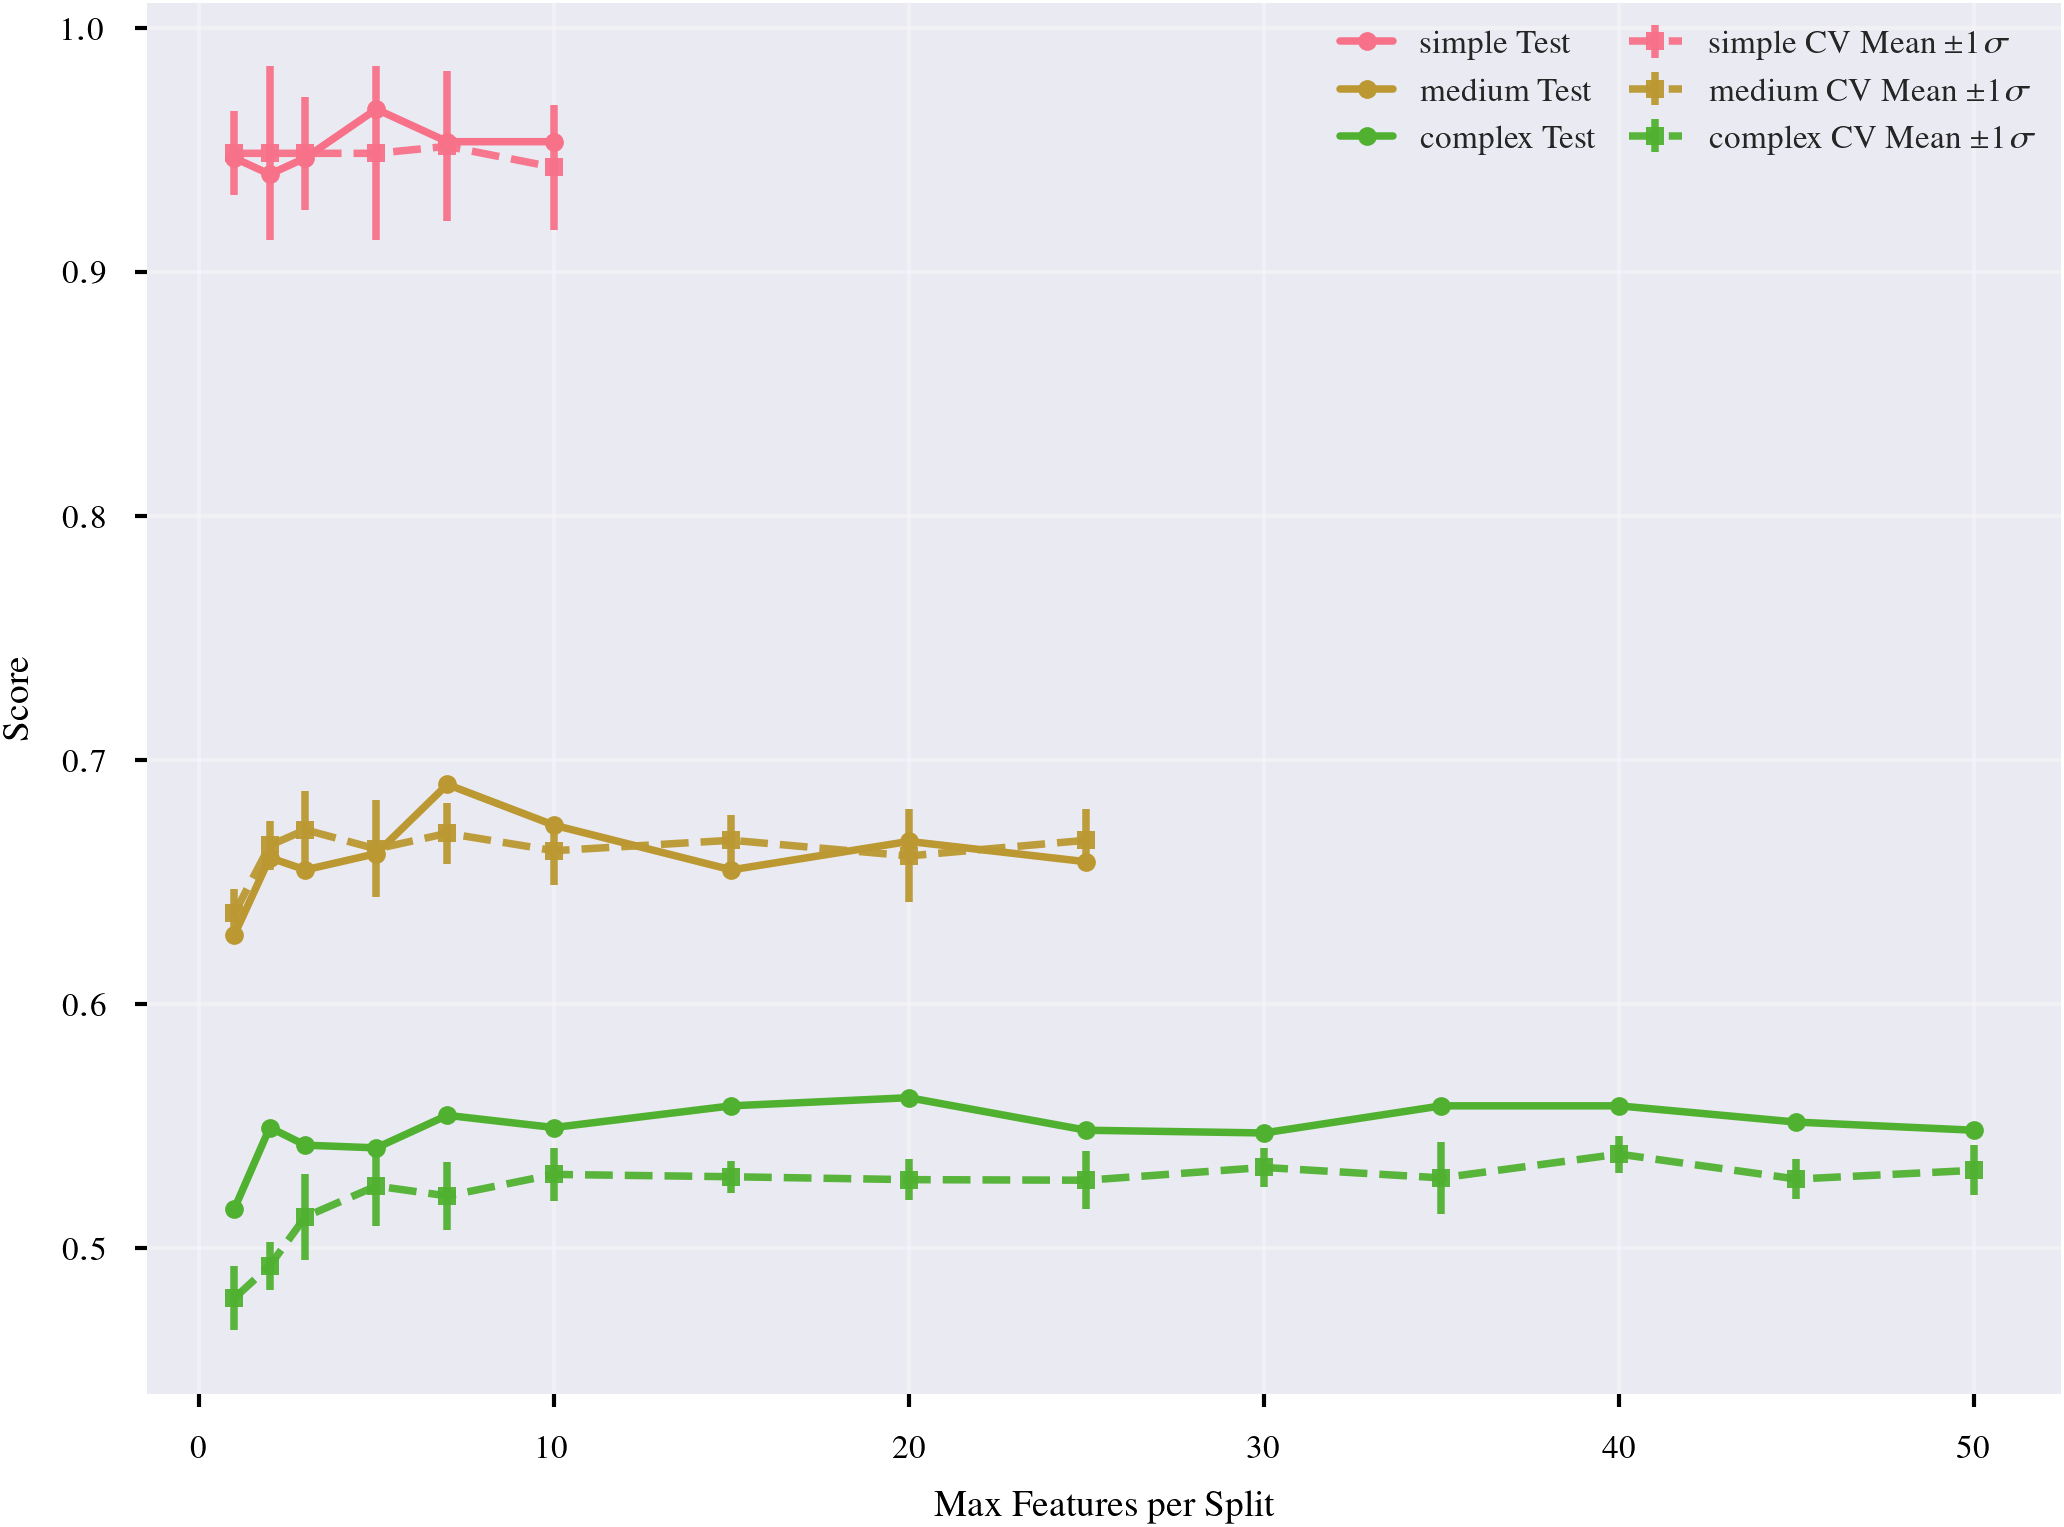
\includegraphics[width=\linewidth]{images/all_datasets_accuracy_vs_features.png}
    \caption{Medium: Test and CV accuracy vs. max\_features.}
    \label{fig:exp2-medium-acc}
  \end{subfigure}
  \caption{Number of features per split vs.\ accuracy (example).}
  \label{fig:exp2-accuracy-features}
\end{figure}


\textbf{Discussion:}
The results in Figure~\ref{fig:exp2-medium-acc} illustrate how varying the number of features considered at each split affects test and cross-validated accuracy. As the number of features increase, there is only a slight improvement in accuracy up to a point, after which the performance does not show any clear signs of improvement. Since each individual tree was allowed to grow deep, the benefit of considering more features at each split gets mitigated by the increased correlation between trees. The correlation reduces the effectiveness of bagging, as the ensemble relies on diverse predictions from its members to reduce variance. Therefore, while increasing the number of features per split can enhance the strength of individual trees, it also increases their similarity, which can limit the ensemble's overall performance. Overall, the findings highlight the nuanced role of feature subsampling in random forests, where both too few and too many features can hinder performance due to underfitting or over-correlation among trees.

\subsection{Experiment 3: Depth vs Number of Trees}
\label{sec:results-exp3}
The heatmaps show a clear interaction between depth and ensemble size: deeper trees require more trees to stabilize variance, while extra trees deliver diminishing returns once variance is averaged out. Accuracy concentrates along a ridge where both parameters are sufficient; increasing one without the other beyond this region offers little benefit, marking natural plateaus.

\begin{figure}[H]
  \centering
  \begin{subfigure}[b]{\columnwidth}
    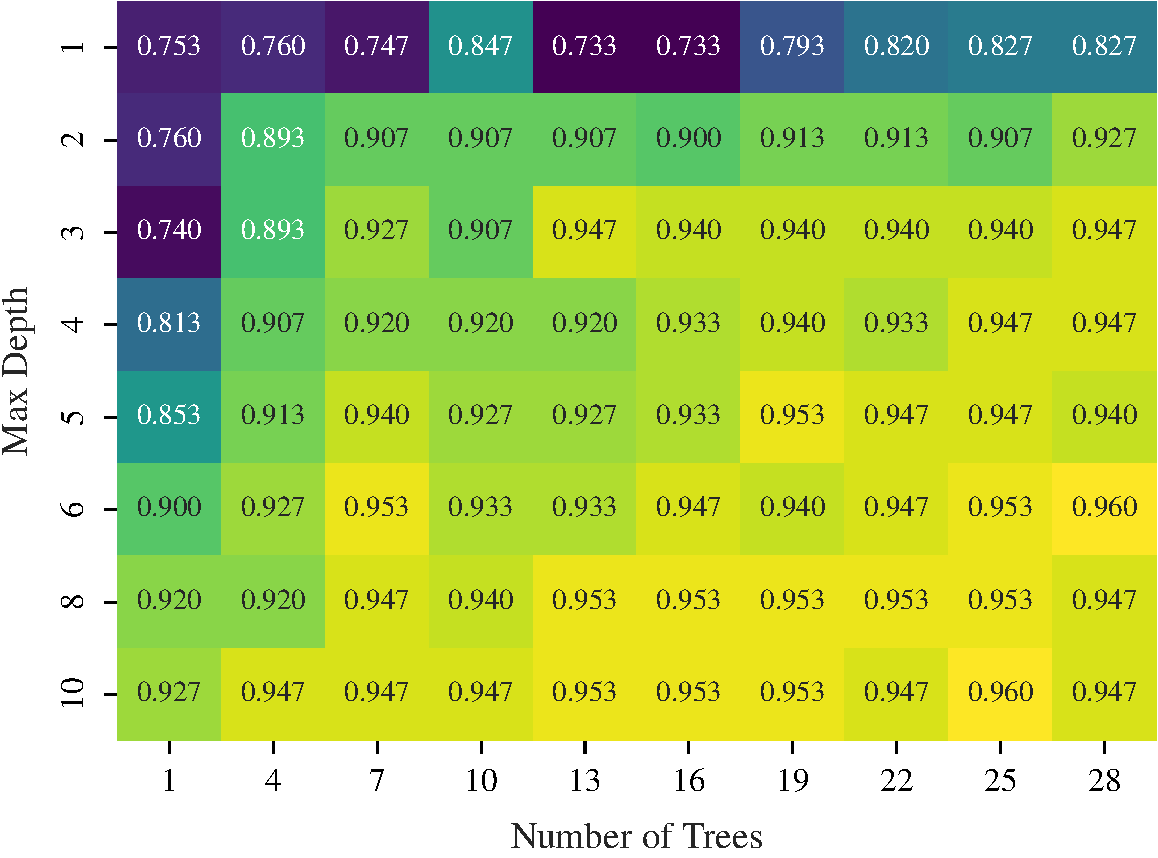
\includegraphics[width=\linewidth]{images/simple_depth_vs_trees_heatmap.pdf}
    \caption{Simple}
    \label{fig:exp3-simple-heatmap-a}
  \end{subfigure}\hfill

  \begin{subfigure}[b]{\columnwidth}
    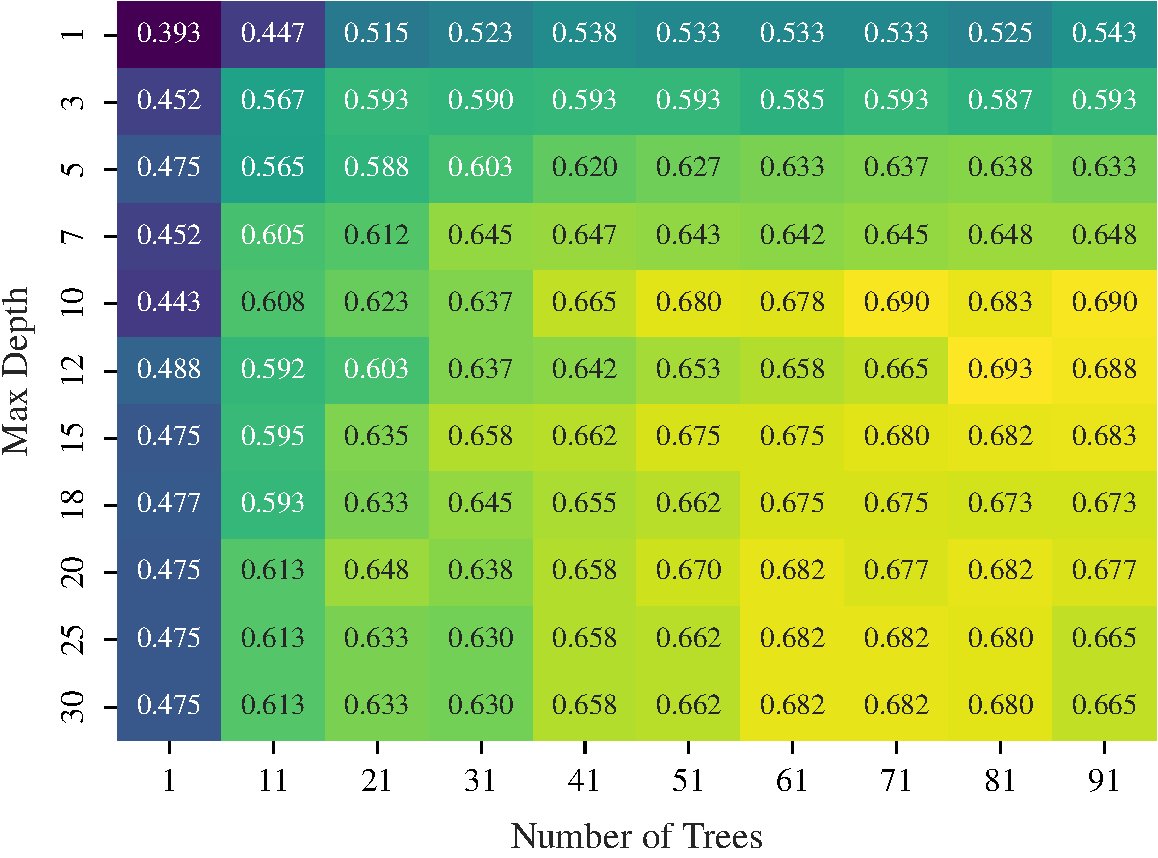
\includegraphics[width=\linewidth]{images/medium_depth_vs_trees_heatmap.pdf}
    \caption{Medium}
    \label{fig:exp3-medium-heatmap}
  \end{subfigure}\hfill
  \begin{subfigure}[b]{\columnwidth}
    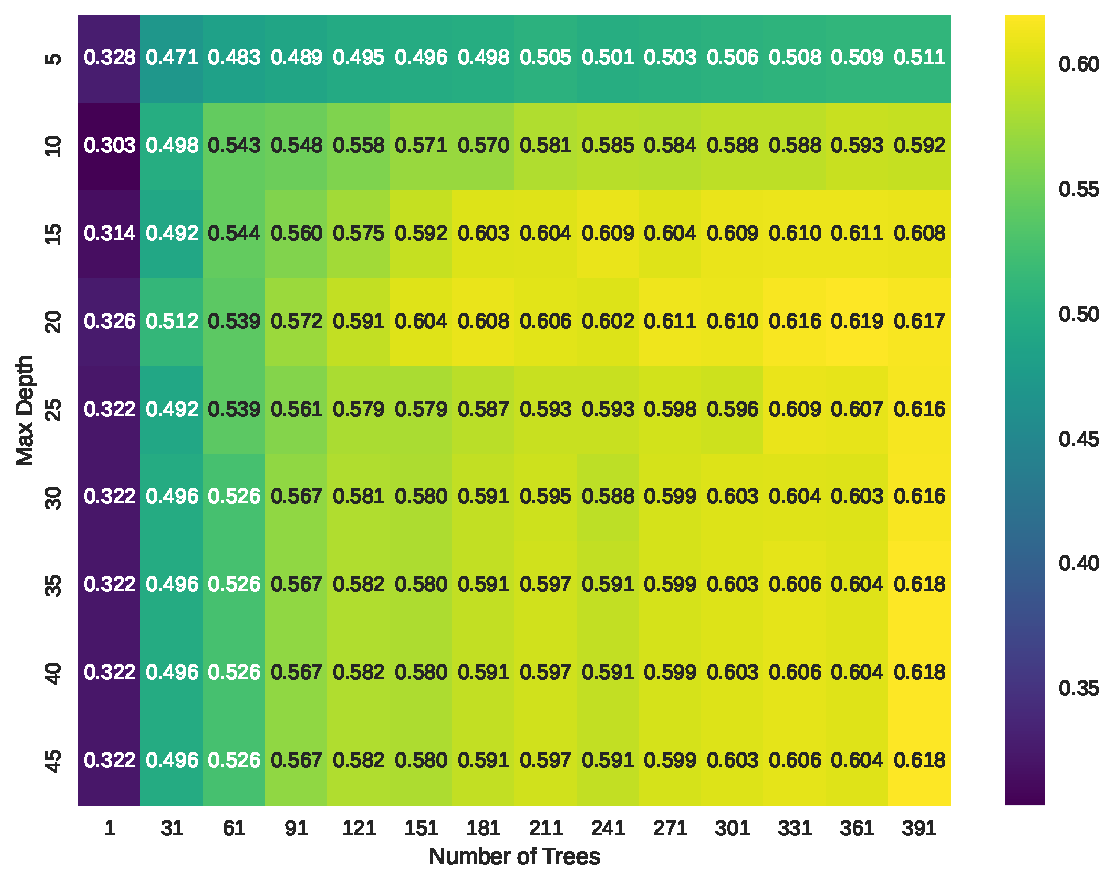
\includegraphics[width=\linewidth]{images/complex_depth_vs_trees_heatmap.pdf}
    \caption{Complex}
    \label{fig:exp3-complex-heatmap}
  \end{subfigure}

  \caption{Heatmaps of test accuracy over maximum tree depth vs.\ number of trees for each dataset.}
  \label{fig:exp3-depth-trees-heatmaps}
\end{figure}

\textbf{Discussion:}

  Each heatmap in Figure~\ref{fig:exp3-depth-trees-heatmaps} has the same pattern - there is a clear relationship between the number of trees in the ensemble and the maximum depth of the trees in the forest. Each heatmap shows a convergence to an optimal configuration. The forest created is dependent on the max depth as seen in Experiment~1, but the performance is also dependent on the number of trees. The results show that even when increasing the max depth, the best results come from increasing the number of trees in conjunction. The general trend shows that more trees in the ensemble and deeper trees both contribute to higher accuracy, which is expected in the case of bagging. The improvement in accuracy with more and deeper trees is due to the overall reduction in variance that bagging provides where, although individual trees may overfit, the ensemble averages out their errors.  

\paragraph{Fixed optimal configurations after Experiment 1-3.} To standardize subsequent comparisons, the following dataset-specific settings were fixed based on the first two experiments and the Experiment~3 ridge regions:
\begin{itemize}
  \item \texttt{optimal\_estimators} = \{\texttt{simple}: 25, \texttt{medium}: 100, \texttt{complex}: 360\}
  \item \texttt{optimal\_depths} = \{\texttt{simple}: 8, \texttt{medium}: 10, \texttt{complex}: 20\}
  \item \texttt{optimal\_num\_split} = \{\texttt{simple}: 5, \texttt{medium}: 7, \texttt{complex}: 15\}
\end{itemize}
These settings are used in Experiment~4 to define the underfit/overfit depth ranges and to hold constant the ensemble size and per-split feature counts.

\subsection{Experiment 4: Mixed-Depth Ensembles}
\label{sec:results-exp4}
The tables compare ensembles mixing underfitted and overfitted trees. Across Simple, Medium, and Complex, the overfit-only composition attains the best test and CV accuracy, indicating that under strong bagging, averaging many high-variance trees outperforms mixing capacities. 

\begin{table}[h]
\centering
\caption{Experiment 4 (Simple): Composition vs.\ accuracy.}
\label{tab:exp4-simple}
\begin{tabular}{lccc}
\toprule
Composition & Train Acc & Test Acc & CV Acc \\
\midrule
Only Underfit      & 0.991 & 0.940 & $0.943 \pm 0.016$ \\
Majority Underfit  & 0.991 & 0.933 & $0.954 \pm 0.028$ \\
Balanced           & 1.000 & 0.960 & $0.946 \pm 0.031$ \\
Majority Overfit   & 1.000 & 0.940 & $0.963 \pm 0.021$ \\
\textbf{Only Overfit}      & \textbf{1.000} & \textbf{0.960} & $\mathbf{0.966 \pm 0.025}$ \\
\bottomrule
\end{tabular}
\end{table}

\begin{table}[h]
\centering
\caption{Experiment 4 (Medium): Composition vs.\ accuracy.}
\label{tab:exp4-medium}
\begin{tabular}{lccc}
\toprule
Composition & Train Acc & Test Acc & CV Acc \\
\midrule
Only Underfit      & 0.969 & 0.655 & $0.669 \pm 0.025$ \\
Majority Underfit  & 0.984 & 0.677 & $0.661 \pm 0.028$ \\
Balanced           & 1.000 & 0.660 & $0.677 \pm 0.019$ \\
Majority Overfit   & 1.000 & 0.652 & $0.672 \pm 0.026$ \\
	\textbf{Only Overfit}      & \textbf{1.000} & \textbf{0.685} & $\mathbf{0.691 \pm 0.021}$ \\
\bottomrule
\end{tabular}
\end{table}

\begin{table}[h]
\centering
\caption{Experiment 4 (Complex): Composition vs.\ accuracy.}
\label{tab:exp4-complex}
\begin{tabular}{lccc}
\toprule
Composition & Train Acc & Test Acc & CV Acc \\
\midrule
Only Underfit      & 1.000 & 0.576 & $0.541 \pm 0.013$ \\
Majority Underfit  & 1.000 & 0.583 & $0.550 \pm 0.015$ \\
Balanced           & 1.000 & 0.595 & $0.550 \pm 0.026$ \\
Majority Overfit   & 1.000 & 0.597 & $0.564 \pm 0.021$ \\
\textbf{Only Overfit}      & \textbf{1.000} & \textbf{0.610} & $\mathbf{0.563 \pm 0.008}$ \\
\bottomrule
\end{tabular}
\end{table}


\textbf{Discussion:}
 The results in Tables~\ref{tab:exp4-simple}, \ref{tab:exp4-medium}, and \ref{tab:exp4-complex} show the performance of ensembles with different compositions of underfitted and overfitted trees across the three datasets. A clear trend emerges where ensembles composed entirely of overfitted trees consistently achieve the highest test accuracy and cross-validated accuracy. The trend suggests that, in the context of bagging, the high variance of overfitted trees is effectively averaged out by the ensemble, leading to better generalization. Mixed compositions do not outperform the all-overfit configuration, indicating that the benefits of averaging high-variance learners outweigh the potential advantages of bias-variance blending through mixed depths. The results are somewhat surprising, as one might expect that a mix of underfitted and overfitted trees would provide a better balance of bias and variance, leading to improved generalization. However, the effectiveness of bagging in reducing variance appears to be sufficient to allow overfitted trees to perform best. With weaker bagging or fewer trees, mixtures may outperform overfit-only. Therefore, it is essential to ensure that there are enough trees within the ensemble to ensure robustness. In another approach, weaker learners could be used exclusively, such as shallow trees, and follow the boosting approach of sequentially correcting errors. However, this would be a different ensemble method and not bagging.

 \subsection{Omnibus and post-hoc statistical tests}
To test for differences among the five ensemble compositions on each dataset, a Friedman test was applied to 35 paired cross-validation blocks, followed by Wilcoxon signed-rank tests which were one-sided and Holm-corrected, comparing the ``Only Overfit'' configuration against each alternative. The omnibus Friedman results were: \textit{simple}: $\chi^2=21.122$, $p=2.995\times10^{-4}$; \textit{medium}: $\chi^2=69.402$, $p=3.035\times10^{-14}$; \textit{complex}: $\chi^2=82.083$, $p=6.302\times10^{-17}$. These indicate statistically significant differences among configurations. Detailed pairwise outcomes are reported in the accompanying notebook.

\begin{table}[h]
\centering
\caption{Post-hoc Wilcoxon vs\ ``Only Overfit'' — \textit{simple} (35 blocks). One-sided alternative tests whether the reference outperforms the comparator; Holm-adjusted p-values control FWER.}
\label{tab:wilcoxon-simple}
\resizebox{\linewidth}{!}{%
\begin{tabular}{lccccc}
\toprule
Comparator & W & p & Holm p & Reject & Mean $\Delta$ Acc \\
\midrule
Only Underfit      & 304.00 & 0.00050 & 0.00199 & True  & 0.01470 \\
Majority Underfit  & 153.50 & 0.03428 & 0.10280 & False & 0.00730 \\
Balanced           & 243.50 & 0.04017 & 0.10280 & False & 0.00570 \\
Majority Overfit   & 179.00 & 0.46420 & 0.46420 & False & 0.00120 \\
\bottomrule
\end{tabular}%
}
\end{table}

\begin{table}[h]
\centering
\caption{Post-hoc Wilcoxon vs\ ``Only Overfit'' — \textit{medium} (35 blocks). One-sided alternative; Holm-adjusted p-values.}
\label{tab:wilcoxon-medium}
\resizebox{\linewidth}{!}{%
\begin{tabular}{lccccc}
\toprule
Comparator & W & p & Holm p & Reject & Mean $\Delta$ Acc \\
\midrule
Only Underfit      & 627.00 & 0.00000 & 0.00000 & True  & 0.03520 \\
Majority Underfit  & 541.50 & 0.00000 & 0.00000 & True  & 0.02130 \\
Balanced           & 562.50 & 0.00000 & 0.00001 & True  & 0.01710 \\
Majority Overfit   & 363.50 & 0.00349 & 0.00349 & True  & 0.00950 \\
\bottomrule
\end{tabular}%
}
\end{table}

\begin{table}[h]
\centering
\caption{Post-hoc Wilcoxon vs\ ``Only Overfit'' — \textit{complex} (35 blocks). One-sided alternative; Holm-adjusted p-values.}
\label{tab:wilcoxon-complex}
\resizebox{\linewidth}{!}{%
\begin{tabular}{lccccc}
\toprule
Comparator & W & p & Holm p & Reject & Mean $\Delta$ Acc \\
\midrule
Only Underfit      & 595.00 & 0.00000 & 0.00000 & True  & 0.02860 \\
Majority Underfit  & 610.50 & 0.00000 & 0.00000 & True  & 0.01950 \\
Balanced           & 581.00 & 0.00001 & 0.00001 & True  & 0.01150 \\
Majority Overfit   & 519.50 & 0.00040 & 0.00040 & True  & 0.00770 \\
\bottomrule
\end{tabular}%
}
\end{table}

\paragraph{Discussion of post-hoc results.} On the \textit{simple} dataset, ``Only Overfit'' is significantly better than ``Only Underfit'' after Holm correction, with Holm $p=0.001989$, while gains over the other three compositions are not statistically significant where mean accuracy deltas are small (\(\approx0.1\%\)–\(1.5\%\)). The other configurations are not significantly different from each other because the problem is small and relatively easy. Trees saturate quickly, and their structures become highly similar across compositions. Strong bagging further reduces variance, so fold-wise paired differences fall within sampling noise. Refer to Table~\ref{tab:wilcoxon-simple} for details.\\

On the \textit{medium} dataset, ``Only Overfit'' significantly outperforms all four alternatives under the one-sided Wilcoxon with Holm adjustment, with Holm $p<0.004$, with effect sizes from \(\approx0.9\%\) to \(3.5\%\), indicating a robust advantage as task complexity increases. Refer to Table~\ref{tab:wilcoxon-medium} for the medium dataset details.\\

On the \textit{complex} dataset, ``Only Overfit'' significantly outperforms all four alternatives with p-values less than 0.05 for all comparisons, corroborating the Friedman omnibus and aligning with the Experiment~\ref{sec:results-exp4} test/CV summaries. Refer to Table~\ref{tab:wilcoxon-complex} for details.


\section{Conclusion}

The assignment investigated how random forest performance is controlled by maximum tree depth, the number of features considered per split, and ensemble size across three datasets of increasing complexity. A reproducible pipeline was implemented with stratified splits, per-tree seeding, and 5-fold cross-validation, and four experiments were conducted: (i) depth sweeps, (ii) feature-subsampling per split sweeps at near-optimal depth, (iii) depth-by-trees interaction grids, and (iv) ensembles mixing under- and overfitting trees.

The main findings are consistent with bias-variance theory and answer the following:
\begin{itemize}
  \item Maximum depth: Test and cross-validated accuracy increase from shallow to moderate depths, then plateau or decline as overfitting emerges. The depth that maximizes generalization increases with task complexity. With sufficiently many trees, deeper models become more viable because bagging reduces variance.
  \item Features per split: Allowing more features strengthens individual trees but raises inter-tree correlation. Accuracy improves to a plateau, after which gains are marginal or flat.
  \item Depth vs.\ ensemble size: There is a trend for better performance where both depth and number of trees are sufficiently large enough and tuned to the dataset complexity. Deeper trees require more trees to stabilize variance. The parameters are limited by each other, where increasing one without the other beyond a certain point yields little benefit.
  \item Mixed-depth ensembles: Under strong bagging, ensembles composed solely of overfitted trees matched or outperformed mixed-capacity ensembles on test and CV accuracy, with comparable or smaller gaps. When ensembles are small or bagging is weak, mixing capacities may be more beneficial.
\end{itemize}

The following practical suggestions emerges from these results: (i) pick depth by maximizing CV performance; (ii) grow the number of trees until CV mean stabilizes and its variance shrinks, noting that deeper forests require more trees; and (iii) when using sufficiently many trees with bagging, homogeneous deep ensembles are a strong baseline.

Limitations and future work: the study used synthetic, balanced datasets and focused on accuracy where if extending to real-world datasets, additional metrics, and class imbalance would broaden conclusions. Secondly, exploring other ensemble methods like boosting or stacking could reveal different dynamics. Finally, investigating interactions with other hyperparameters such as minimum samples per leaf or pruning would provide a more comprehensive understanding of random forest tuning.
Overall, the best configurations balance depth, feature subsampling, and ensemble size, with preferred values growing with task complexity. Under strong bagging, larger ensembles of deeper trees generally deliver the most stable and accurate performance.


 The associated code for all the calculations.
\footnote{The code for this report is available on GitHub: \url{https://github.com/grantxxcoder/25849646rw441Assignment4}.}.
\appendix

\section*{List of Acronyms}
\begingroup
\setlength{\tabcolsep}{6pt}
\renewcommand{\arraystretch}{1.05}
\noindent\begin{tabular}{@{}p{0.22\columnwidth}p{0.75\columnwidth}@{}}
\textbf{Acronym} & \textbf{Definition} \\
\midrule
CV & Cross-validation \\
\end{tabular}
\endgroup

% References
\bibliographystyle{apalike}
\bibliography{references}

\end{document}
